\documentclass[11pt,a4paper]{article}

% These are extra packages that you might need for writing the equations:
\usepackage{amsmath}
\usepackage{amsfonts}
\usepackage{amssymb}
\usepackage{booktabs}
\usepackage{hyperref}
\usepackage{listings}
\usepackage{xcolor}
\usepackage{graphicx}
\usepackage{subfig}
\usepackage{float}
\usepackage{outlines}

\lstset {language=C++,
		 basicstyle=\ttfamily,
         keywordstyle=\color{blue}\ttfamily,
         stringstyle=\color{red}\ttfamily,
         commentstyle=\color{purple}\ttfamily,
         morecomment=[l][\color{magenta}]{\#},
       	 basicstyle=\tiny}

% You need the following package in order to include figures in your report:
\usepackage{graphicx}

% With this package you can set the size of the margins manually:
\usepackage[left=2cm,right=2cm,top=2cm,bottom=2cm]{geometry}


\begin{document}

% Enter the exercise number, your name and date here:
\noindent\parbox{\linewidth}{
 \parbox{.25\linewidth}{ \large ICP, Exercise 07 }\hfill
 \parbox{.5\linewidth}{\begin{center} \large Beat Hubmann \end{center}}\hfill
 \parbox{.2\linewidth}{\begin{flushright} \large Nov 11, 2018 \end{flushright}}
}
\noindent\rule{\linewidth}{2pt}




\section{Introduction}

A limited diffusion aggregation (DLA) algorithm was implemented on a 2D lattice.
The aggregation behaviour for different simulation parameters was observed.

\section{Algorithm Description}
The algorithm was implemented in continuous space with wraparound borders and a central aggregation seed.
Random walking particles change heading and speed at each step. Their coordinates get projected to the lattice only
when checking for coalescence. Particles enter the system at a random location on the lattice border (i.e. on any of the 
four sides). To limit simulation time, particle lifetime is a simulation parameter; if no contact with the aggregating cluster
is made after this set amount of steps, the particle expires and a new one is launched.\\
The algorithm works along the following principle:
\begin{outline}
    \1 for $n$ particles do:
     \2 randomly pick starting site along lattice boundary
     \2 randomly pick starting heading
     \2 while not in direct vicinity of aggreggating cluster and while age smaller than lifetime do:
        \3 randomly change heading
        \3 randomly change velocity
        \3 walk one timestep to new position
        \3 check and record cluster vicinity
        \3 increase age
    \1 draw final lattice state 

\end{outline}

\section{Results}

The program was implemented as described above and submitted with this report. 
As expected, the cluster grows outward from the seed in random tree-like structures. The occupation probability grows 
as the cluster grows toward the lattice edges containing the release points (see figure~\ref{fig:1} as an example).\\

Applying 'noise reduction' by requiring $m$ visits to a site before the site gets occupied makes the cluster denser with
increasing $m$ (see figure~\ref{fig:2}).


\begin{figure}
\begin{center}
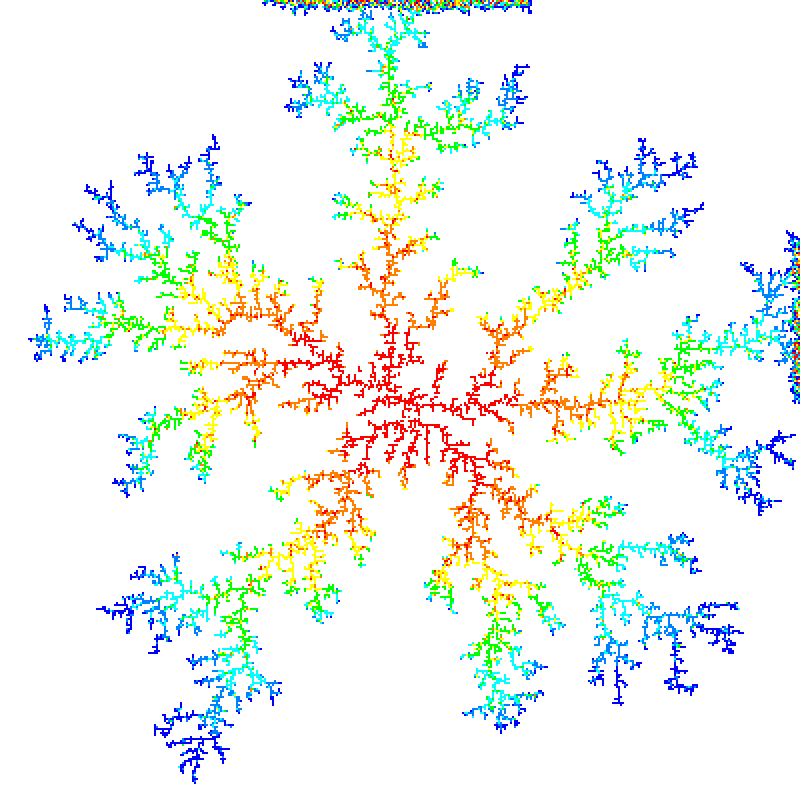
\includegraphics[scale=0.4]{fig_1.png} 
\end{center}
\caption{DLA cluster on 2D lattice with side length $L=400$, particle lifetime $100000$ steps, particle count $20000$, noise reduction $m=0$, center seed.}
\label{fig:1}
\end{figure}

\begin{figure}
    \begin{center}
    \begin{tabular}{cc}
    \subfloat[m=2]{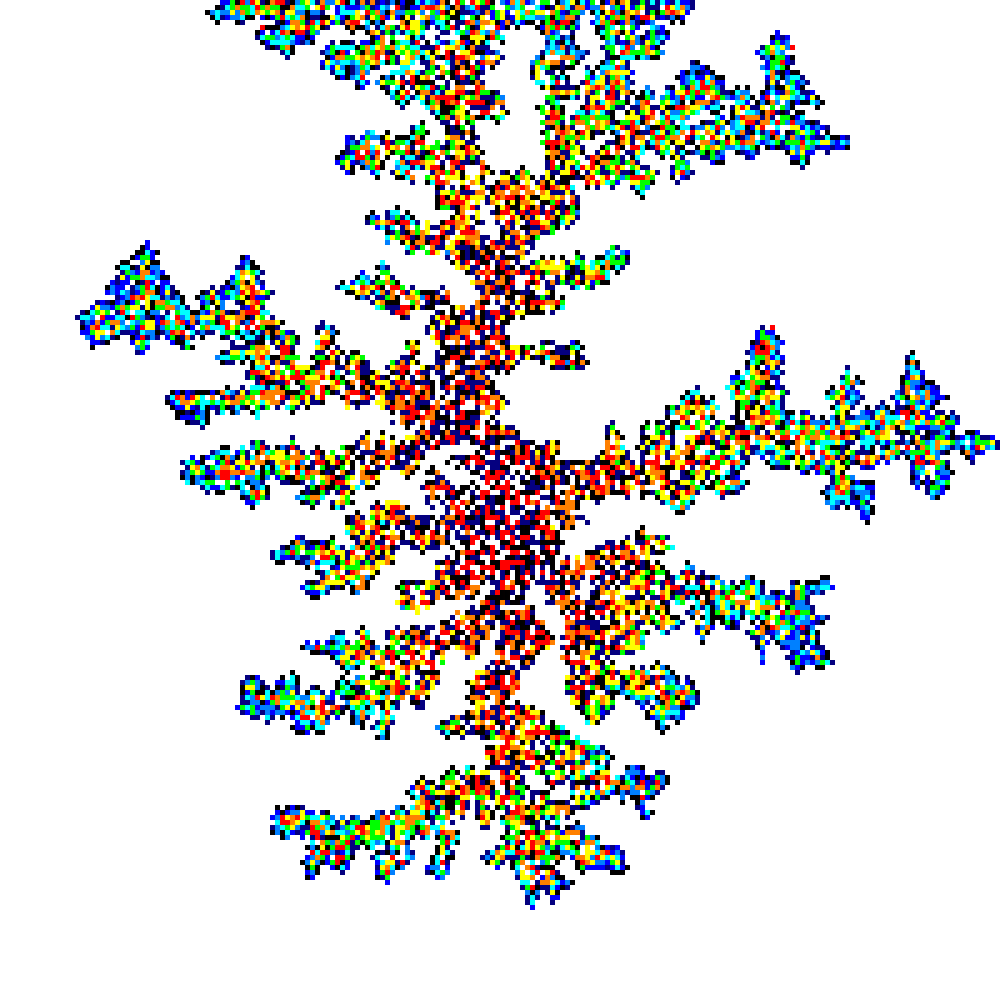
\includegraphics[width = 2.0in]{fig_2_0.png}} &
    \subfloat[m=4]{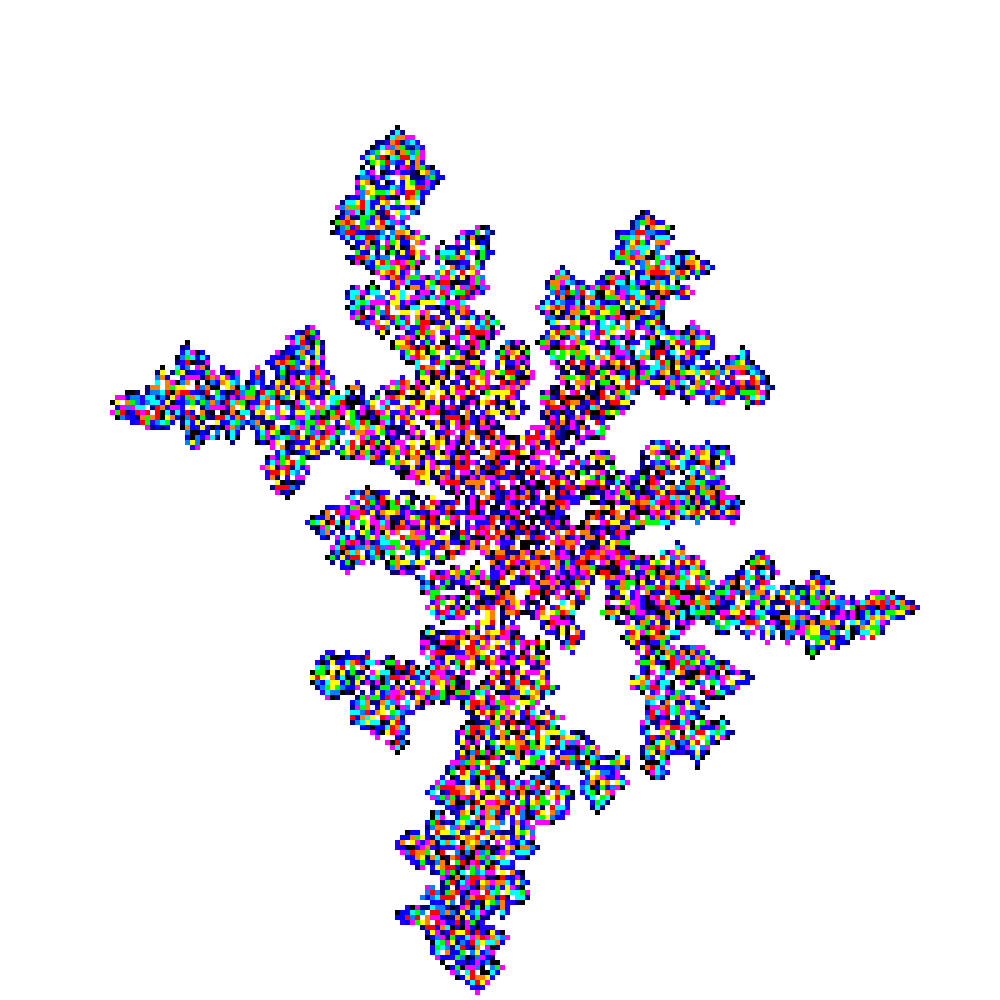
\includegraphics[width = 2.0in]{fig_2_1.png}} \\
    \subfloat[m=6]{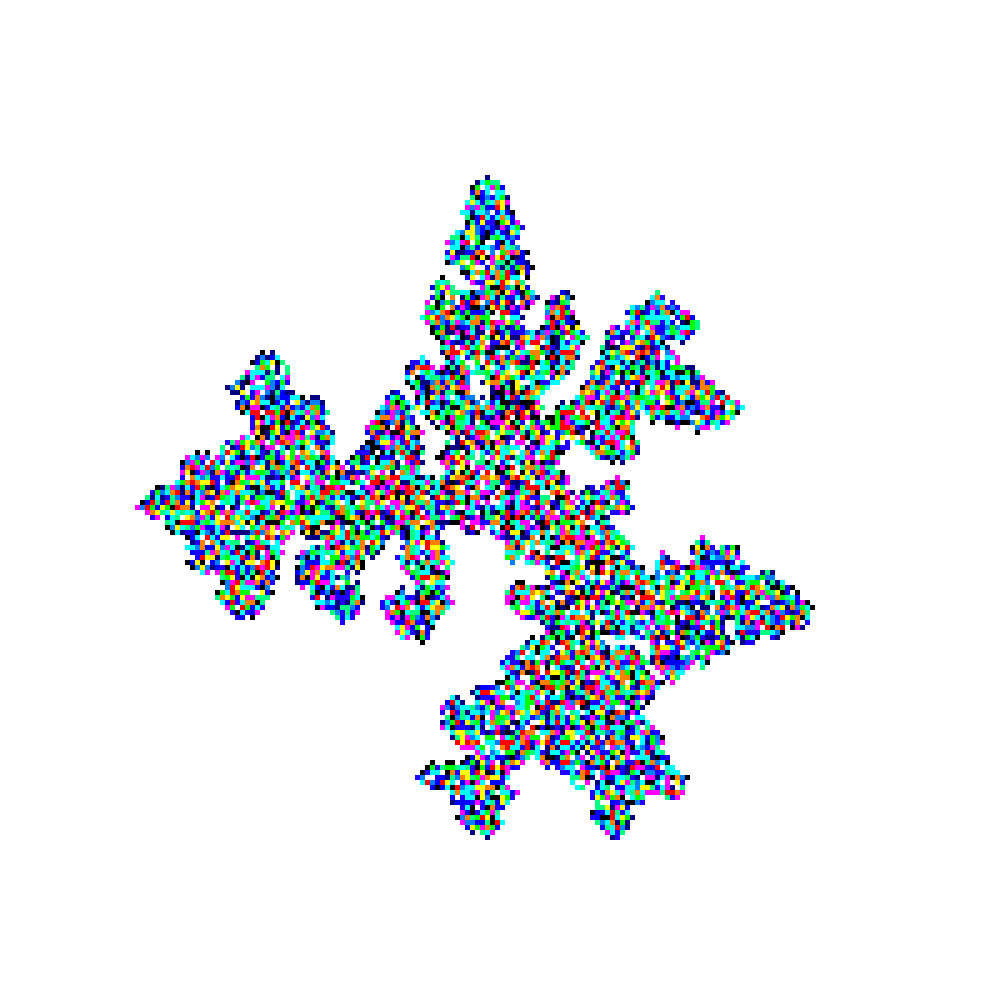
\includegraphics[width = 2.0in]{fig_2_2.png}} & 
    \subfloat[m=8]{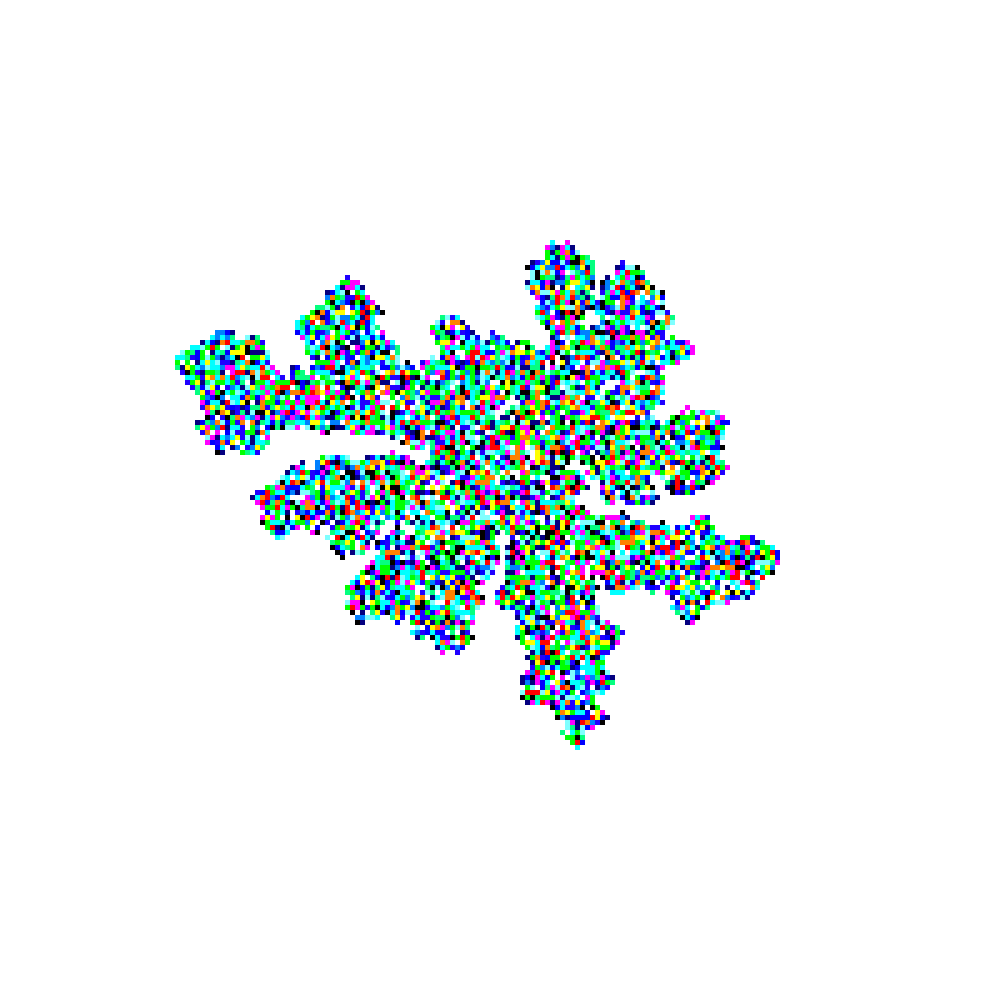
\includegraphics[width = 2.0in]{fig_2_3.png}} 
    \end{tabular}
\end{center}
    \caption{Different noise reduction parameters $m$ for DLA cluster on 2D lattice with side length $L=200$, particle lifetime $100000$ steps, particle count $10000$, center seed.}
\label{fig:2}
\end{figure}


\section{Discussion}
In general, the algorithm yields the results expected from theory. As I wanted to go for 'true' randomness and not inject
particles near the cluster boundary as suggested by the task statement to improve runtime, rather long lifetimes were necessary for particles to be
reasonbly likely to make it to the center seed.


\pagebreak
\begin{thebibliography}{99}


\bibitem{herrmann}
	Herrmann, H. J.,
	Singer, H. M.,
	Mueller L.,
	Buchmann, M.-A.,\\
	\emph{Introduction to Computational Physics - Lecture Notes},\\
	ETH Zurich,\\
	2017.


\end{thebibliography}

\end{document}